\documentclass[twoside,11pt,a4paper]{article}

\usepackage[utf8]{inputenc}
\usepackage{mathtools}
\usepackage{latexsym}
\usepackage{amsmath}
\usepackage{amssymb}




\usepackage[left=2cm,right=2cm,top=2cm,bottom=2cm]{geometry}
\usepackage{tikz}
\usetikzlibrary{decorations.pathreplacing}
\usetikzlibrary{fadings}

%% \usepackage{natbib}
\usepackage[backend=bibtex,style=authoryear]{biblatex}
\addbibresource{~/Cloud/library/catalog.bib}

%% \usepackage[lf]{venturis}
%% \usepackage[T1]{fontenc}


\definecolor{lightblue}{rgb}{0.65,0.78,0.92}
\definecolor{lightgreen}{rgb}{0.62,0.88,0.58}
\definecolor{lightpurple}{rgb}{0.87,0.61,.93}
\definecolor{lightorange}{rgb}{0.95,0.82,0.58}
\definecolor{lightgray}{rgb}{0.8,0.8,0.8}


% args = position, width, height, depth, color, top label, bottom label
\newcommand{\drawcnnlayer}[7]{
  \path (0,0);
  \begin{scope}[shift={#1}]
  \draw[black,fill=#5] (0,0,0) -- ++(-#2,0,0) -- ++(0,-#3,0) -- ++(#2,0,0) -- cycle;
  \draw[black,fill=#5] (0,0,0) -- ++(0,0,-#4) -- ++(0,-#3,0) -- ++(0,0,#4) -- cycle;
  \draw[black,fill=#5] (0,0,0) -- ++(-#2,0,0) -- ++(0,0,-#4) -- ++(#2,0,0) -- cycle;
  %% \node at (0,#4) {#6};
  %% \node at (0,-#4) {#7};
  \end{scope}
}


\title{Model Information and Architectures}
\author{Patrick Sullivan}


\begin{document}

\maketitle

\section{Variational Autoencoder}

The model implemented here is essentially as introduced in (\cite{kingma2013auto}). It uses the ``reparameterization trick'' to construct a
Gaussian noise sampling that is differentiable, enabling us to backprop the loss over the entire network. The network is trained
end-to-end with a single loss function

\begin{equation}
\mathcal{L}(\textbf{x}) =
\underbrace{\frac{1}{n} \sum_i^n \textbf{x} \log{\hat{\textbf{x}}} + (1-\textbf{x}) \log{(1-\hat{\textbf{x}})}}_{\text{reconstruction error}} +
\underbrace{\frac{1}{2n} \sum_i^n \mu^2 + \sigma^2 - \log{\sigma^2} - 1}_{\text{latent loss}}
\end{equation}

The loss function encourages the network to encode the input into a value that is consistent with being sampled from a Guassian distribution,
while encouraging the decoder to translate this encoding to an image that matches the original.
By encouraging the encoding to follow a Guassian distribution, we can then sample from it, feed this value to the decoder, and create new
generative outputs. 


See Fig. \ref{fig:vae-encoder} and Fig. \ref{fig:vae-decoder} for the encoder and decoder architecture, respectively.


\begin{figure}
  \begin{center}
    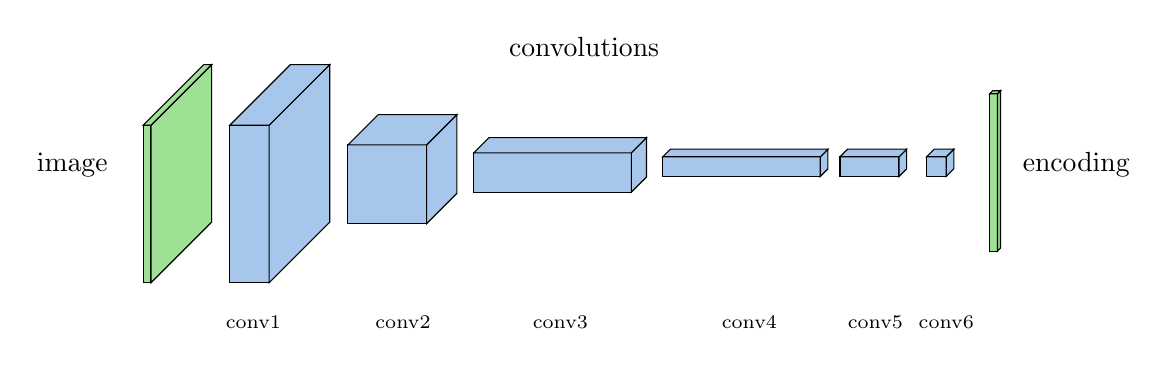
\begin{tikzpicture}
      \node at (-1,-.5) {image};
      \drawcnnlayer{(0,0)}{0.1}{2}{2}{lightgreen}{image}{};
      \node at (5.5,1) {convolutions};
      \node at (1.3,-2.5) {\scriptsize{conv1}};
      \drawcnnlayer{(1.5,0)}{0.5}{2}{2}{lightblue}{conv1}{5:2\#64};
      \node at (3.2,-2.5) {\scriptsize{conv2}};
      \drawcnnlayer{(3.5,-0.25)}{1.0}{1}{1}{lightblue}{conv2}{5:2\#128};
      \node at (5.2,-2.5) {\scriptsize{conv3}};
      \drawcnnlayer{(6.1,-0.35)}{2.0}{0.5}{0.5}{lightblue}{conv3}{5:2\#256};
      \node at (7.6,-2.5) {\scriptsize{conv4}};
      \drawcnnlayer{(8.5,-0.4)}{2.0}{.25}{.25}{lightblue}{conv4}{5:2\#256};
      \node at (9.2,-2.5) {\scriptsize{conv5}};
      \drawcnnlayer{(9.5,-0.4)}{0.75}{0.25}{0.25}{lightblue}{conv5}{32x32:1\#96};
      \node at (10.1,-2.5) {\scriptsize{conv6}};
      \drawcnnlayer{(10.1,-0.4)}{0.25}{0.25}{0.25}{lightblue}{conv6}{32x32:1\#32};
      \drawcnnlayer{(10.75,0.4)}{0.1}{2}{0.1}{lightgreen}{logits}{};
      \node at (11.75,-.5) {encoding};
    \end{tikzpicture}

    \vspace{1em}


    \begin{tabular}{l||l|l|l}
      layer & filter size & stride & \# filters \\
      \hline
      conv1 & 5 & 2 & 64 \\
      conv2 & 5 & 2 & 128 \\
      conv3 & 5 & 2 & 256 \\
      conv4 & 5 & 2 & 256 \\
      \hline
      conv5 & 32 & 1 & 96 \\
      conv6 & 32 & 1 & 32
    \end{tabular}

    \caption{\textbf{VAE encoder} architecture. All layers use Leaky ReLU activations. The final convolution output is flattened and represents our encoded image.}
  \end{center}
  \label{fig:vae-encoder}
\end{figure}

\begin{figure}
  \begin{center}
    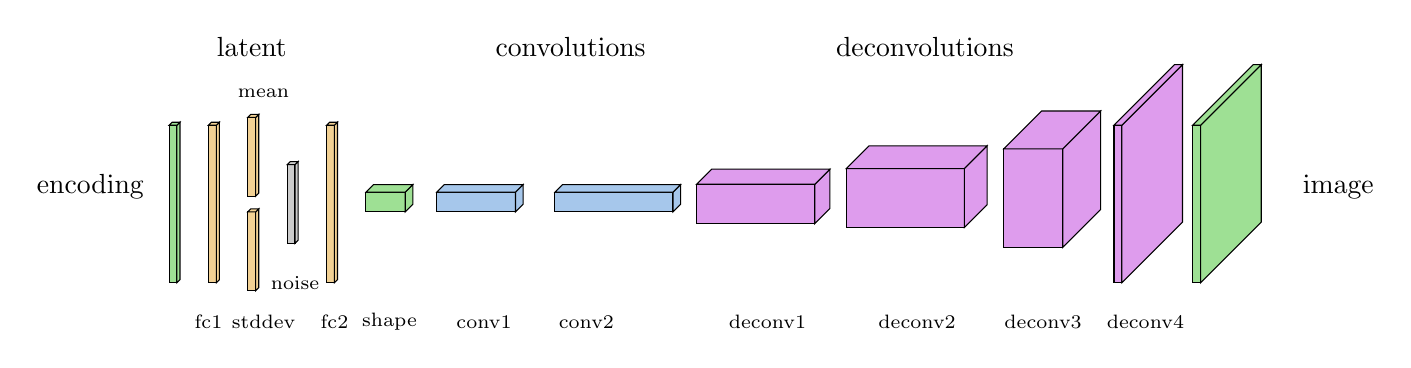
\begin{tikzpicture}
      \node at (-1.1,-.78) {encoding};
      %% \node at (-.1,-2.54) {\scriptsize{n}};
      \drawcnnlayer{(0,0)}{0.1}{2}{0.1}{lightgreen}{}{};

      
      \node at (0.95,1) {latent};
      \node at (0.40,-2.5) {\scriptsize{fc1}};
      \drawcnnlayer{(0.5,0)}{0.1}{2}{0.1}{lightorange}{}{};

      \node at (1.1,.4) {\scriptsize{mean}};
      \drawcnnlayer{(1,.1)}{0.1}{1}{0.1}{lightorange}{}{};

      \node at (1.1,-2.5) {\scriptsize{stddev}};
      \drawcnnlayer{(1,-1.1)}{0.1}{1}{0.1}{lightorange}{}{};
      
      \node at (1.5,-2) {\scriptsize{noise}};
      \drawcnnlayer{(1.5,-.5)}{0.1}{1}{0.1}{lightgray}{}{};      

      \node at (2,-2.5) {\scriptsize{fc2}};
      \drawcnnlayer{(2.0,0)}{0.1}{2}{0.1}{lightorange}{}{};      
      
      \node at (2.7,-2.5) {\scriptsize{shape}};            
      \drawcnnlayer{(2.9,-0.85)}{0.5}{0.25}{0.25}{lightgreen}{}{};
      
      
      \node at (5,1) {convolutions};
      \node at (3.9,-2.5) {\scriptsize{conv1}};
      \drawcnnlayer{(4.3,-0.85)}{1}{0.25}{0.25}{lightblue}{}{};
      \node at (5.2,-2.5) {\scriptsize{conv2}};      
      \drawcnnlayer{(6.3,-0.85)}{1.5}{0.25}{0.25}{lightblue}{}{};

      \node at (9.5,1) {deconvolutions};
      \node at (7.5,-2.5) {\scriptsize{deconv1}};
      \drawcnnlayer{(8.1,-0.75)}{1.5}{0.5}{0.5}{lightpurple}{}{};
      
      \node at (9.4,-2.5) {\scriptsize{deconv2}};      
      \drawcnnlayer{(10.0,-0.55)}{1.5}{.75}{.75}{lightpurple}{}{};
      \node at (11,-2.5) {\scriptsize{deconv3}};      
      \drawcnnlayer{(11.25,-0.3)}{0.75}{1.25}{1.25}{lightpurple}{}{};
      \node at (12.3,-2.5) {\scriptsize{deconv4}};
      \drawcnnlayer{(12,0)}{0.1}{2}{2}{lightpurple}{}{};

      \drawcnnlayer{(13,0)}{0.1}{2}{2}{lightgreen}{}{};
      \node at (14.75,-.78) {image};
    \end{tikzpicture}

    \vspace{1em}


    \begin{tabular}{l||l|l|l}
      layer & filter size & stride & \# filters (or size) \\
      \hline
      fc1 & & & 512 \\
      stddev & & & 200 \\
      mean & & & 200 \\
      noise & & & 200 \\
      fc2 & & & 512 \\
      shape & & & 4x4x32\\
      \hline
      conv1 & 1 & 1 & 96 \\
      conv2 & 1 & 1 & 256 \\
      \hline
      deconv1 & 5 & 2 & 256 \\
      deconv2 & 5 & 2 & 128 \\
      deconv3 & 5 & 2 & 64 \\            
      deconv4 & 5 & 2 & 3 \\     
      
    \end{tabular}

    
  \end{center}
  \caption{\textbf{VAE decoder} architecture. The latent is generated by remapping the encoding into two vectors representing the \emph{mean} and the \emph{standard deviation} of a Gaussian, which is then (via the reparameterization trick) used to generate a Gaussian. This is then mapped back out through a dense layer before reshaping into a small, but deep, image. This is then run through two convolution filters to expand the number of filters before upscaling with deconvolution operations.}
  \label{fig:vae-decoder}  
\end{figure}


\section{Standard, Wasserstein, and Improved Wasserstein GANs}

There are a few different GANs implemented that share the same architecture but differ in how they are trained. They are:

\begin{itemize}
\item Standard GAN (\cite{goodfellow2014generative})
\item Wasserstein GAN (\cite{arjovsky2017wasserstein})
\item Improved Wasserstein GAN (\cite{gulrajani2017improved})
\end{itemize}

See Fig. \ref{fig:gan-generator} and Fig. \ref{fig:gan-discriminator} for the generator and discriminator architectures, respectively.

\subsection{Standard GAN}

In a standard GAN, the generator is trained against the loss function
\begin{equation}
  \mathcal{L}(\textbf{x}) = \frac{1}{n}\sum_i^n - \log(\text{disc}(\text{gen}(\textbf{x})))
\end{equation}


while the discriminator is trained against

\begin{equation}
  \mathcal{L}(\textbf{x}) = \frac{1}{n}\sum_i^n - \log(\text{disc}(\textbf{x})) - \log(1 - \text{disc}(\text{gen}(\textbf{x})))
\end{equation}


The discriminator is trained $t > 0$ times in sequence followed by training the generator once.






\begin{figure}
  \begin{center}
    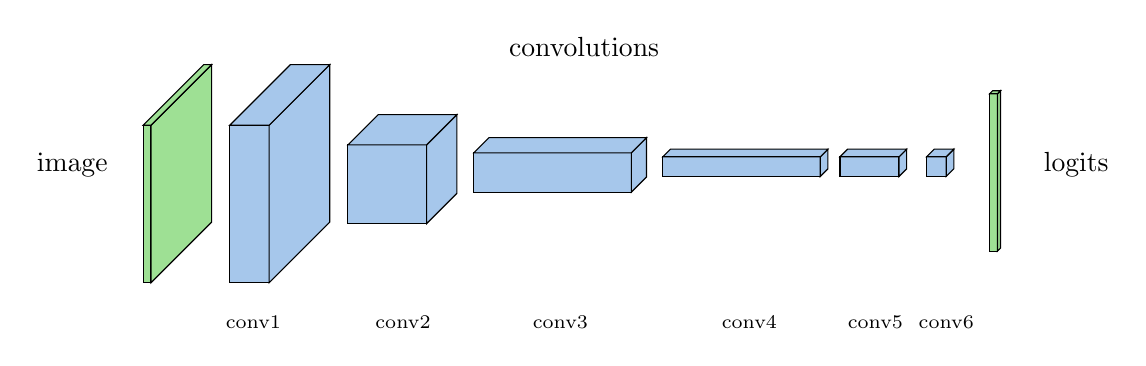
\begin{tikzpicture}
      \node at (-1,-.5) {image};
      \drawcnnlayer{(0,0)}{0.1}{2}{2}{lightgreen}{image}{};
      \node at (5.5,1) {convolutions};
      \node at (1.3,-2.5) {\scriptsize{conv1}};
      \drawcnnlayer{(1.5,0)}{0.5}{2}{2}{lightblue}{conv1}{5:2\#64};
      \node at (3.2,-2.5) {\scriptsize{conv2}};
      \drawcnnlayer{(3.5,-0.25)}{1.0}{1}{1}{lightblue}{conv2}{5:2\#128};
      \node at (5.2,-2.5) {\scriptsize{conv3}};
      \drawcnnlayer{(6.1,-0.35)}{2.0}{0.5}{0.5}{lightblue}{conv3}{5:2\#256};
      \node at (7.6,-2.5) {\scriptsize{conv4}};
      \drawcnnlayer{(8.5,-0.4)}{2.0}{.25}{.25}{lightblue}{conv4}{5:2\#256};
      \node at (9.2,-2.5) {\scriptsize{conv5}};
      \drawcnnlayer{(9.5,-0.4)}{0.75}{0.25}{0.25}{lightblue}{conv5}{32x32:1\#96};
      \node at (10.1,-2.5) {\scriptsize{conv6}};
      \drawcnnlayer{(10.1,-0.4)}{0.25}{0.25}{0.25}{lightblue}{conv6}{32x32:1\#32};
      \drawcnnlayer{(10.75,0.4)}{0.1}{2}{0.1}{lightgreen}{logits}{};
      \node at (11.75,-.5) {logits};
    \end{tikzpicture}

    \vspace{1em}


    \begin{tabular}{l||l|l|l}
      layer & filter size & stride & \# filters \\
      \hline
      conv1 & 5 & 2 & 64 \\
      conv2 & 5 & 2 & 128 \\
      conv3 & 5 & 2 & 256 \\
      conv4 & 5 & 2 & 256 \\
      \hline
      conv5 & 32 & 1 & 96 \\
      conv6 & 32 & 1 & 32
    \end{tabular}
  \end{center}

  \caption{\textbf{GAN/WGAN discriminator} architecture. In the original GAN/WGAN architecture, all convolution layers use batch normalization and a leaky ReLU activation function. In the improved WGAN architecture, batch norm is omitted. All three models use \emph{sigmoid} activation in the logits layer.}
  \label{fig:gan-discriminator}
\end{figure}



\begin{figure}
  \begin{center}
    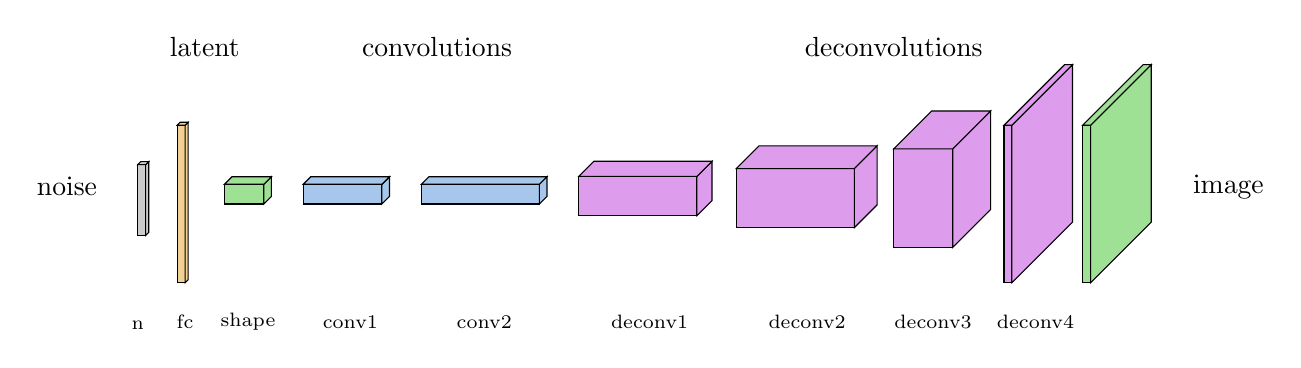
\begin{tikzpicture}
      \node at (-1,-.78) {noise};
      \node at (-.1,-2.54) {\scriptsize{n}};      
      \drawcnnlayer{(0,-.5)}{0.1}{.9}{0.1}{lightgray}{}{};
      \node at (0.75,1) {latent};
      \node at (0.50,-2.5) {\scriptsize{fc}};      
      \drawcnnlayer{(0.5,0)}{0.1}{2}{0.1}{lightorange}{}{};
      \node at (1.3,-2.5) {\scriptsize{shape}};            
      \drawcnnlayer{(1.5,-0.75)}{0.5}{0.25}{0.25}{lightgreen}{}{};
      
      
      \node at (3.7,1) {convolutions};
      \node at (2.6,-2.5) {\scriptsize{conv1}};
      \drawcnnlayer{(3.0,-0.75)}{1}{0.25}{0.25}{lightblue}{}{};
      \node at (4.3,-2.5) {\scriptsize{conv2}};      
      \drawcnnlayer{(5.0,-0.75)}{1.5}{0.25}{0.25}{lightblue}{}{};

      \node at (9.5,1) {deconvolutions};
      \node at (6.4,-2.5) {\scriptsize{deconv1}};
      \drawcnnlayer{(7.0,-0.65)}{1.5}{0.5}{0.5}{lightpurple}{}{};
      \node at (8.4,-2.5) {\scriptsize{deconv2}};      
      \drawcnnlayer{(9.0,-0.55)}{1.5}{.75}{.75}{lightpurple}{}{};
      \node at (10,-2.5) {\scriptsize{deconv3}};      
      \drawcnnlayer{(10.25,-0.3)}{0.75}{1.25}{1.25}{lightpurple}{}{};
      \node at (11.3,-2.5) {\scriptsize{deconv4}};
      \drawcnnlayer{(11,0)}{0.1}{2}{2}{lightpurple}{}{};

      \drawcnnlayer{(12,0)}{0.1}{2}{2}{lightgreen}{}{};
      \node at (13.75,-.78) {image};
    \end{tikzpicture}

    \vspace{1em}

    \begin{tabular}{l||l|l|l}
      layer & filter size & stride & \# filters (or size) \\
      \hline
      n & & & 200 \\
      fc & & & 512 \\
      shape & & & 4x4x32 \\
      \hline
      conv1 & 1 & 1 & 96 \\
      conv2 & 1 & 1 & 256 \\
      \hline
      deconv1 & 5 & 2 & 256 \\
      deconv2 & 5 & 2 & 128 \\
      deconv3 & 5 & 2 & 64 \\            
      deconv4 & 5 & 2 & 3 \\
      
    \end{tabular}

    
  \end{center}
  \caption{\textbf{GAN/WGAN generator} architecture. Starting with a latent vector of Gaussian noise, we expand it using a fully connected layer and then reshape it into an image with depth. The number of filters is then expanded further using convolutions before upscaling it several times using deconvolution operations. Each (de)convolution layer uses batch normalization and a ReLU activation function, and the final output values are rescaled with \emph{tanh}.}
  \label{fig:gan-generator}
\end{figure}




%input:  64x64x3
%        32x32x64
%        16x16x128
%        8x8x256
%        4x4x256
%        4x4x96
%latent: 4x4x32
%        4x4x96
%        4x4x256
%        8x8x156
%        16x16x128
%        32x32x64
%output: 64x64x1


\section{Conditional WGAN}

This model is actually neither conditional nor a GAN, however, it bears several similaries. It is a combination of the ``pix2pix'' model described in (\cite{isola2016image}) and the Improved Wasserstein training techniques found in (\cite{gulrajani2017improved}).


See Fig. \ref{fig:cgan-generator} and Fig. \ref{fig:cgan-discriminator} for the generator and discriminator architecture, respectively.

\begin{figure}
  \begin{center}
    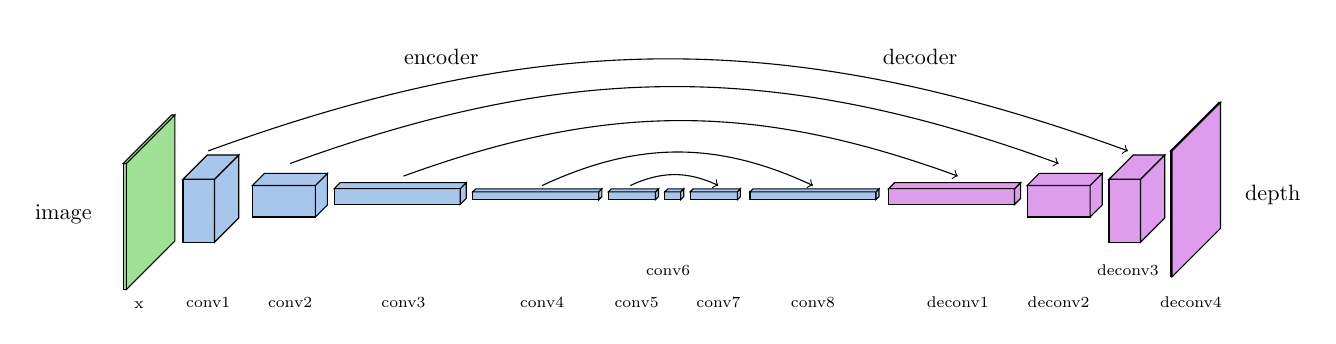
\begin{tikzpicture}[scale=0.8,every node/.style={scale=0.8}]
      \node at (4,1.2) {encoder};
      \node at (11.6,1.2)  {decoder};
      \node at (-2.0,-1.3) {image};
      \drawcnnlayer{(-1,-.5)}{0.05}{2}{2}{lightgreen}{}{};        % 64x64x3
      \node at (-0.8,-2.75) {\scriptsize{x}};
      
      \drawcnnlayer{(0.4,-.75)}{0.5}{1}{1}{lightblue}{}{};          % 32x32x64
      \node at (0.3,-2.7) {\scriptsize{conv1}};
      \coordinate (I) at (0.3, -.30);
      
      \drawcnnlayer{(2.0,-.85)}{1}{0.5}{0.5}{lightblue}{}{};        % 16x16x128
      \node at (1.6,-2.7) {\scriptsize{conv2}};
      \coordinate (G) at (1.6,-.50);
      
      \drawcnnlayer{(4.3,-.90)}{2}{0.25}{0.25}{lightblue}{}{};      % 8x8x256
      \node at (3.4,-2.7) {\scriptsize{conv3}};
      \coordinate (E) at (3.4,-.70);
      
      \drawcnnlayer{(6.5,-.95)}{2}{0.125}{0.125}{lightblue}{}{};    % 4x4x256
      \node at (5.6,-2.7) {\scriptsize{conv4}};
      \coordinate (C) at (5.6,-.85);
      
      \drawcnnlayer{(7.4,-.95)}{0.75}{0.125}{0.125}{lightblue}{}{}; % 4x4x96
      \node at (7.1,-2.7) {\scriptsize{conv5}};
      \coordinate (A) at (7.0, -.85);
      
      \drawcnnlayer{(7.8,-.95)}{0.25}{0.125}{0.125}{lightblue}{}{}; % 4x4x32
      \node at (7.6,-2.2) {\scriptsize{conv6}};
      
      \drawcnnlayer{(8.7,-.95)}{0.75}{0.125}{0.125}{lightblue}{}{}; % 4x4x96
      \node at (8.4,-2.7) {\scriptsize{conv7}};
      \coordinate (B) at (8.4,-.85);
      \draw [->] (A) to [bend left=25] node [midway,above]{} (B);
      
      \drawcnnlayer{(10.9,-.95)}{2}{0.125}{0.125}{lightblue}{}{};   % 4x4x256
      \node at (9.9,-2.7) {\scriptsize{conv8}};
      \coordinate (D) at (9.9,-.85);
      \draw [->] (C) to [bend left=25] node [midway,above]{} (D);

      
      \drawcnnlayer{(13.1,-.90)}{2}{0.25}{0.25}{lightpurple}{}{};   % 8x8x256
      \node at (12.2,-2.7) {\scriptsize{deconv1}};
      \coordinate (F) at (12.2,-.70);
      \draw [->] (E) to [bend left=20] node [midway,above]{} (F);      
      
      \drawcnnlayer{(14.3,-.85)}{1}{0.5}{0.5}{lightpurple}{}{};     % 16x16x128
      \node at (13.8,-2.7) {\scriptsize{deconv2}};
      \coordinate (H) at (13.8,-.50);
      \draw [->] (G) to [bend left=20] node [midway,above]{} (H);            
      
      \drawcnnlayer{(15.1,-.75)}{0.5}{1}{1}{lightpurple}{}{};       % 32x32x64
      \node at (14.9,-2.2) {\scriptsize{deconv3}};
      \coordinate (J) at (14.9, -.30);
      \draw [->] (I) to [bend left=20] node [midway,above]{} (J);                  
      
      \drawcnnlayer{(15.6,-.3)}{0.025}{2}{2}{lightpurple}{}{};      % 64x64x1
      \node at (15.9,-2.7) {\scriptsize{deconv4}};
      \node at (17.2, -1.0) {depth};
    \end{tikzpicture}

    \vspace{1em}

    \begin{tabular}{l||l|l|l}
      layer & filter size & stride & \# filters (or size) \\
      \hline
      x & & & 64x646x3 \\
      conv1 & 5 & 2 & 64 \\
      conv2 & 5 & 2 & 128 \\
      conv3 & 5 & 2 & 256 \\
      conv4 & 5 & 2 & 256 \\
      conv5 & 1 & 1 & 96 \\
      \hline
      conv6 & 1 & 1 & 32 \\
      \hline
      conv7 & 1 & 1 & 96 + skip\\
      conv8 & 1 & 1 & 256 + skip\\
      deconv1 & 5 & 2 & 256 + skip\\
      deconv2 & 5 & 2 & 128 + skip\\
      deconv3 & 5 & 2 & 64 + skip\\
      deconv4 & 5 & 2 & 1 \\
    \end{tabular}


  \end{center}
  \caption{
    \textbf{cGAN generator} architecture.
    A 64x64x3 RGB image is passed into the network and is then encoded into a 512-sized latent vector (conv6).
    This is then decoded back out to a 64x64x1 image representing an estimation of the depth.
    Skip layers are added from each layer in the encoder to its match in the decoder via concatenation.
    Activations in the generator are LeakyReLU while the decoder uses ReLU, with the final layer using tanh.
    If enabled, batchnorm and dropout occurs at all layers except the first and last layers.
    The loss for this network is
    \begin{equation}
      \mathcal{L(\textbf{x})} = \frac{1}{n}\sum_i^n \text{disc}(\text{gen}(\textbf{x})) + \frac{1}{n}\sum_i^n \sqrt{(\textbf{x}-\hat{\textbf{x}})^2}
    \end{equation}
    aka the Wasserstein loss from the discriminator plus the RMSE loss of the reconstructed depth.}
  
  \label{fig:cgan-generator}
\end{figure}

%input:  64x64x4
%        32x32x64
%        16x16x128
%        8x8x256
%        8x8x512,
%output: 8x8x1, sigmoid

\begin{figure}
  \begin{center}
    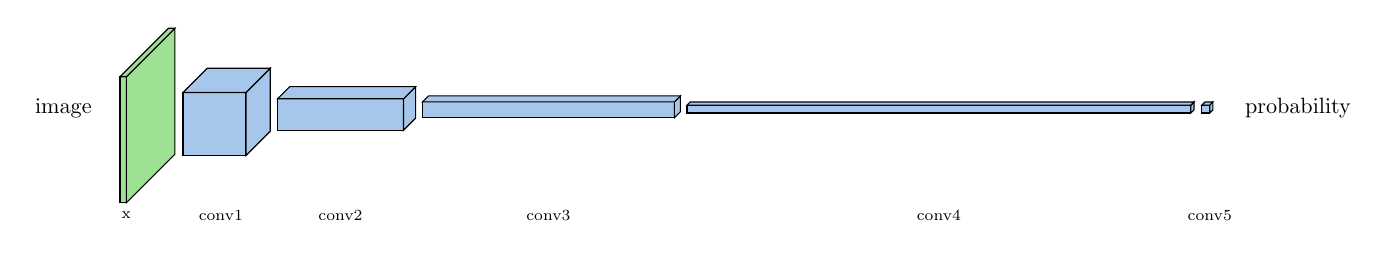
\begin{tikzpicture}[scale=0.8,every node/.style={scale=0.8}]
      \node at (-1,-1) {image};
      \node at (18.6,-1) {probability};
      \drawcnnlayer{(0,-.5)}{0.1}{2}{2}{lightgreen}{}{};
      \node at (0,-2.7) {\scriptsize{x}};
      
      \drawcnnlayer{(1.9,-.75)}{1.0}{1}{1}{lightblue}{}{};
      \node at (1.5,-2.7) {\scriptsize{conv1}};
      
      \drawcnnlayer{(4.4,-.85)}{2.0}{0.5}{0.5}{lightblue}{}{};
      \node at (3.4,-2.7) {\scriptsize{conv2}};
      
      \drawcnnlayer{(8.7,-.90)}{4.0}{0.25}{0.25}{lightblue}{}{};
      \node at (6.7,-2.7) {\scriptsize{conv3}};
      
      \drawcnnlayer{(16.9,-.95)}{8.0}{0.125}{0.125}{lightblue}{}{};
      \node at (12.9,-2.7) {\scriptsize{conv4}};
      
      \drawcnnlayer{(17.2,-.95)}{0.125}{0.125}{0.125}{lightblue}{}{};
      \node at (17.2,-2.7) {\scriptsize{conv5}};      
    \end{tikzpicture}

     \vspace{1em}

    \begin{tabular}{l||l|l|l}
      layer & filter size & stride & \# filters (or size) \\
      \hline
      x & & & 64x64x4 \\
      conv1 & 5 & 2 & 64 \\
      conv2 & 5 & 2 & 128 \\
      conv3 & 5 & 2 & 256 \\
      conv4 & 1 & 1 & 512 \\
      conv5 & 1 & 1 & 1 \\
    \end{tabular}


  \end{center}
  \caption{\textbf{cGAN discriminator} architecture.
    This is a standard DCGAN architecture that takes a 64x64x4 image (RGB concatenated with depth) and returns a single probability as to whether the input is fake or real.
    Activations are LeakyReLU, with the exception of the final layer, which uses sigmoid.
    The loss for this network is
    \begin{equation}
      \mathcal{L}(\textbf{x}) = \frac{1}{n}\sum_i^n \text{disc}(\text{gen}(\textbf{x})) - \frac{1}{n}\sum_i^n \text{disc}(\textbf{x}) + \lambda P
    \end{equation}
    where $P$ is the gradient penalty from \cite{gulrajani2017improved}.
  }
  \label{fig:cgan-discriminator}
\end{figure}


\newpage
\section{Bibliography}
\printbibliography
\end{document}



